\section{Classification Methods}\label{paperA:sec:classification-methods}

We here describe the classification methods and approaches that we have used to provide benchmark results to the dataset. We apply both deterministic deep neural networks as well as a deep generative model used for representation learning to the natural images that we have collected. Furthermore, we utilize the additional information -- iconic images -- from our dataset with a multi-view deep generative model. This model can utilize different data sources and obtain superior representation quality as well as high interpretability. For a fair evaluation, we use a linear classifier with the learned representation from the different methods.

\paragraph*{Deep Neural Networks.} 
CNNs have been the state-of-the-art models in image classification ever since AlexNet \citeA{paperA:krizhevsky2012imagenet} achieved the best classification accuracy in ILSVRC in 2012.
However, in general, computer vision models require lots of labeled data to achieve satisfactory performance, which has resulted in interest for adapting CNNs that have already been trained on a large amount of training data to other image datasets. When adapting pretrained CNNs to new datasets, we can either use it directly as a feature extractor, a.k.a use the off-the-shelf features,~\citeA{paperA:donahue2014decaf, paperA:razavian2014cnnfeatures}, or fine-tune it~\citeA{paperA:Girshick2014rich-feature-hierarchies, paperA:oquab2014learning-and-transferring, paperA:pan2010transferlearning, paperA:yosinski2014transferable, paperA:Zhang2014PartbasedRCNN}. Using off-the-shelf features, we need to specify which feature representation we should extract from the network and use these for training a new classifier. Fine-tuning a CNN involves adjusting the pretrained model parameters, such that the network can e.g. classify images from a dataset different from what the CNN was trained on before. We can either choose to fine-tune the whole network or select some layer parameters to adjust while keeping the others fixed. One important factor on deciding which approach to choose is the size of the new dataset and how similar the new dataset is to the dataset which the CNN was previously trained on. A rule of thumb here is that the closer the features are to the classification layer, the features become more specific to the training data and task \citeA{paperA:yosinski2014transferable}. 

Using off-the-shelf CNN features and fine-tuned CNNs have been successfully applied in \citeA{paperA:donahue2014decaf, paperA:razavian2014cnnfeatures} and \citeA{paperA:Girshick2014rich-feature-hierarchies, paperA:oquab2014learning-and-transferring, paperA:Zhang2014PartbasedRCNN} respectively.
In \citeA{paperA:donahue2014decaf, paperA:razavian2014cnnfeatures}, it is shown that the pretrained features have sufficient representational power to generalize well to other visual recognition tasks with simple linear classifiers, such as Support Vector Machines (SVMs), without fine-tuning the parameters of the CNN to the new task. In \citeA{paperA:Girshick2014rich-feature-hierarchies, paperA:Zhang2014PartbasedRCNN}, all CNN parameters are fine-tuned, whereas in \citeA{paperA:oquab2014learning-and-transferring} the pretrained CNN layer parameters are kept fixed and only an adaptation layer of two fully connected layers are trained on the new task. The results from these works motivate why we should evaluate our dataset on fine-tuned CNNs or linear classifiers trained on off-the-shelf feature representations instead of training an image recognition model from scratch. 

\vspace{-3mm}
\paragraph{Variational Autoencoders with only natural images.}
Deep generative models, 
e.g. the variational autoencoder (VAE)~\citeA{paperA:kingma2014autoencoding, paperA:Rezende2014StochasticBA, paperA:zhang2017advances}, have become widely used in the machine learning community thanks to their generative nature. We thus use VAEs for representation learning as the second benchmarking method. For efficiency, we use low-level pretrained features from a CNN as inputs to the VAE.

The latent representations from VAEs are encodings of the underlying factors for how the data are generated. VAEs belongs to the family of latent variable models, which commonly has the form $p_{\boldsymbol{\theta}}(\mathbf{x},\mathbf{z}) = p(\mathbf{z}) p_{\boldsymbol{\theta}}(\mathbf{x}|\mathbf{z})$, where $p(\mathbf{z})$ is a prior distribution over the latent variables $\mathbf{z}$ and $p_{\boldsymbol{\theta}}(\mathbf{x}|\mathbf{z})$ is the likelihood over the data $\mathbf{x}$ given $\mathbf{z}$. The prior distribution is often assumed to be Gaussian,
$p(\mathbf{z}) = \mathcal{N}(\mathbf{z}\,|\, \boldsymbol{0}, \mathbf{I})$,  
whereas the likelihood distribution depends on the values of $\mathbf{x}$.
The likelihood $p_{\boldsymbol{\theta}}(\mathbf{x}|\mathbf{z})$ is referred to as a decoder represented as a neural network parameterized by $\boldsymbol{\theta}$. An encoder network $q_{\boldsymbol{\phi}}(\mathbf{z}|\mathbf{x})$ parameterized by $\boldsymbol{\phi}$ is introduced as an approximation of the true posterior $p_{\boldsymbol{\theta}}(\mathbf{z}|\mathbf{x})$, which is intractable since it requires computing the integral $p_{\boldsymbol{\theta}}(\mathbf{x}) = \int p_{\boldsymbol{\theta}}(\mathbf{x}, \mathbf{z}) \, d\mathbf{z}$. 
When the prior distribution is a Gaussian, the approximate posterior is also modeled as a Gaussian, $q_{\boldsymbol{\phi}}(\mathbf{z}|\mathbf{x}) = \mathcal{N}(\mathbf{z} \,|\,\boldsymbol{\mu}(\mathbf{x}), \boldsymbol{\sigma}^2(\mathbf{x}) \odot \mathbf{I})$, with some mean $\boldsymbol{\mu}(\mathbf{x})$ and variance $\boldsymbol{\sigma}^2(\mathbf{x})$ computed by the encoder network. The goal is to maximize the marginal log-likelihood by defining a lower bound using $q_{\boldsymbol{\phi}}(\mathbf{z}|\mathbf{x})$:
\begin{align}
\begin{split}\label{eq:vae-loss}
\log p_{\boldsymbol{\theta}}(\mathbf{x}) \geq \mathcal{L}(\boldsymbol{\theta}, \boldsymbol{\phi}; \mathbf{x}) = & \mathbb{E}_{q_{\boldsymbol{\phi}}(\mathbf{z}|\mathbf{x})}\left[\, \log p_{\boldsymbol{\theta}}(\mathbf{x} | \mathbf{z}) \,\right] \\ & -D_{KL}(q_{\boldsymbol{\phi}}(\mathbf{z}|\mathbf{x})\,||\,p(\mathbf{z})) .
\end{split}
\end{align}
The last term is the Kullback-Leibler (KL) divergence of the approximate posterior from the true posterior. The lower bound $\mathcal{L}$ is called the evidence lower bound (ELBO) and can be optimized with stochastic gradient descent via backpropagation \citeA{paperA:doersch2016tutorialvae, paperA:kingma2014autoencoding}. 
VAE is a probabilistic framework. Many extensions such as utilizing structured priors\citeA{paperA:butepage2018Inform} or using continual learning \citeA{paperA:nguyen2018variational} have been explored.
%In fully supervised learning settings, we would have to retrain the model when a new class is introduced. 
%Another advantage is that VAEs can be extended to multimodal data and learn joint latent representations between data pairs, such as image--text or image--image. 
In the following method, we describe how to make use of the iconic images while retaining the unsupervised learning setting in VAEs.

\vspace{-3mm}
\paragraph{Utilizing iconic images with multi-view VAEs.}
Utilizing extra information has shown to be useful in many applications with various model designs~\citeA{paperA:butepage2018Inform, paperA:vedantam2018generative, paperA:vinyals2015show, paperA:wang2016vcca, paperA:zhang2016inter}. For computer vision tasks, natural language is the most commonly used modality to aid the visual representation learning. However, the consistency of the language and visual embeddings has no guarantee. As an example with our dataset, the product description of a Royal Gala apple explains the appearance of a red apple. But if the description is represented with word embeddings, e.g. word2vec \citeA{paperA:mikolov2013distributedrepresentations}, the word 'royal' will probably be more similar to the words 'king' and 'queen' than 'apple'. Therefore, if available, additional visual information about objects might be more beneficial for learning meaningful representations instead of text. In this work, with our collected dataset, we propose to utilize the iconic images for the representation learning of natural images using a multi-view VAE. Since the natural images can include background noise and grocery items different from the targeted one, the role of the iconic image will be to guide the model to which features that are of interest in the natural image.

The VAE can be extended to modeling multiple views of data, where a latent variable $\mathbf{z}$ is assumed to have generated the views \citeA{paperA:vedantam2018generative, paperA:wang2016vcca}. Considering two views $\mathbf{x}$ and $\mathbf{y}$, the joint distribution over the paired random variables ($\mathbf{x}$, $\mathbf{y}$) and latent variable $\mathbf{z}$ can be written as $p_{\boldsymbol{\theta}}(\mathbf{x}, \mathbf{y}, \mathbf{z}) = p(\mathbf{z})p_{\boldsymbol{\theta^{(1)}}}(\mathbf{x}\,|\,\mathbf{z})p_{\boldsymbol{\theta^{(2)}}}(\mathbf{y}\,|\,\mathbf{z})$, where both $p_{\boldsymbol{\theta^{(1)}}}(\mathbf{x}\,|\,\mathbf{z})$ and $p_{\boldsymbol{\theta^{(2)}}}(\mathbf{y}\,|\,\mathbf{z})$ are represented as neural networks with parameters $\boldsymbol{\theta^{(1)}}$ and $\boldsymbol{\theta^{(2)}}$. Assuming that the latent variable $\mathbf{z}$ can reconstruct both $\mathbf{x}$ and $\mathbf{y}$ when only $\mathbf{x}$ is encoded into $\mathbf{z}$ by the encoder $q_{\boldsymbol{\phi}}(\mathbf{z}|\mathbf{x})$, then the ELBO is written as 
\begin{align}
\begin{split}\label{eq:vcca-loss}
\log p_{\boldsymbol{\theta}}(\mathbf{x}, \mathbf{y}) \geq & \, \mathcal{L}(\boldsymbol{\theta}, \boldsymbol{\phi}; \mathbf{x}, \mathbf{y}) \\ 
= & \,  \mathbb{E}_{q_{\boldsymbol{\phi}}(\mathbf{z}|\mathbf{x})}\left[\, \log p_{\boldsymbol{\theta^{(1)}}}(\mathbf{x} | \mathbf{z}) + \log p_{\boldsymbol{\theta^{(2)}}}(\mathbf{y} | \mathbf{z}) \,\right] \\ 
& -D_{KL}(q_{\boldsymbol{\phi}}(\mathbf{z}|\mathbf{x})\,||\,p(\mathbf{z})) .
\end{split}
\end{align}  
This model is referred to as variational autoencoder canonical correlation analysis (VAE-CCA) and was introduced in \citeA{paperA:wang2016vcca}. The main motivation for using VAE-CCA is that the latent representations need to contain information about reconstructing both natural and iconic images.
The main motivation for using VAE-CCA is that 
the latent representation needs to preserve information about how both the natural and iconic images are reconstructed. This also allows us to produce iconic images from new natural images to enhance the interpretability of the latent representation of VAE-CCA (see Section \ref{paperA:sec:experimental-results}) \citeA{paperA:vedantam2018generative}.

%\begin{comment}
	
\begin{figure}[t]
    \centering
    \begin{subfigure}[b]{0.35\textwidth}
    	\centering
    	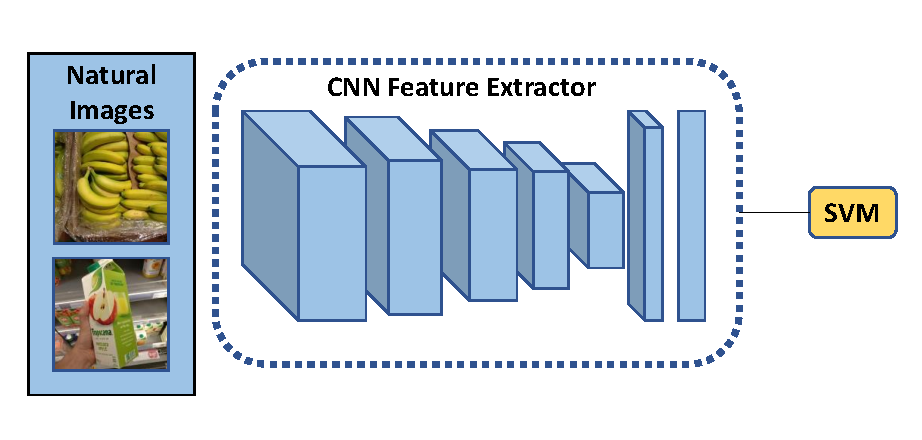
\includegraphics[width=\textwidth]{PaperA/figures/cnn.pdf}
    	%\vspace{-7mm}
    	\caption{}
    	\label{subfig:cnn}
    \end{subfigure} ~
    \begin{subfigure}[b]{0.6\textwidth}
		\centering
		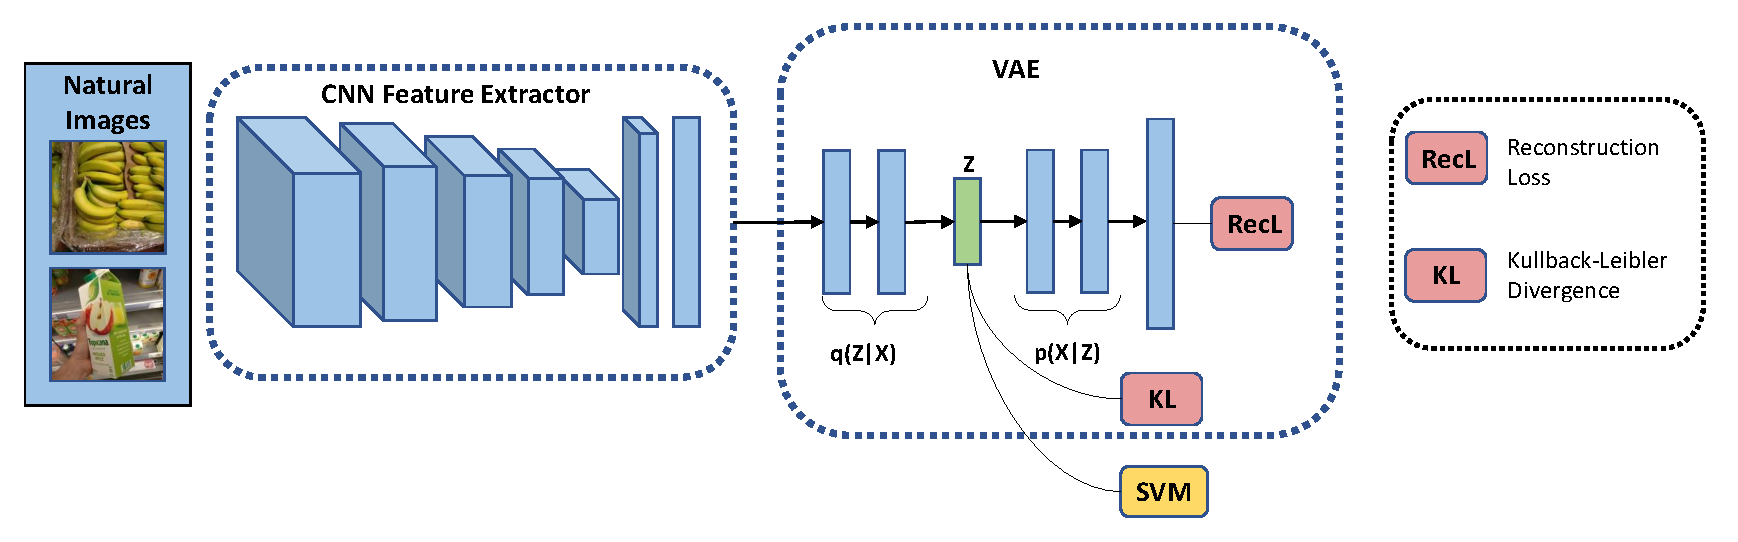
\includegraphics[width=\textwidth]{PaperA/figures/cnn+vae.pdf}
		%\vspace{-7mm}
		\caption{}
		\label{subfig:cnn+vae}
	\end{subfigure} \\
    \begin{subfigure}[b]{0.7\textwidth}
		\centering
		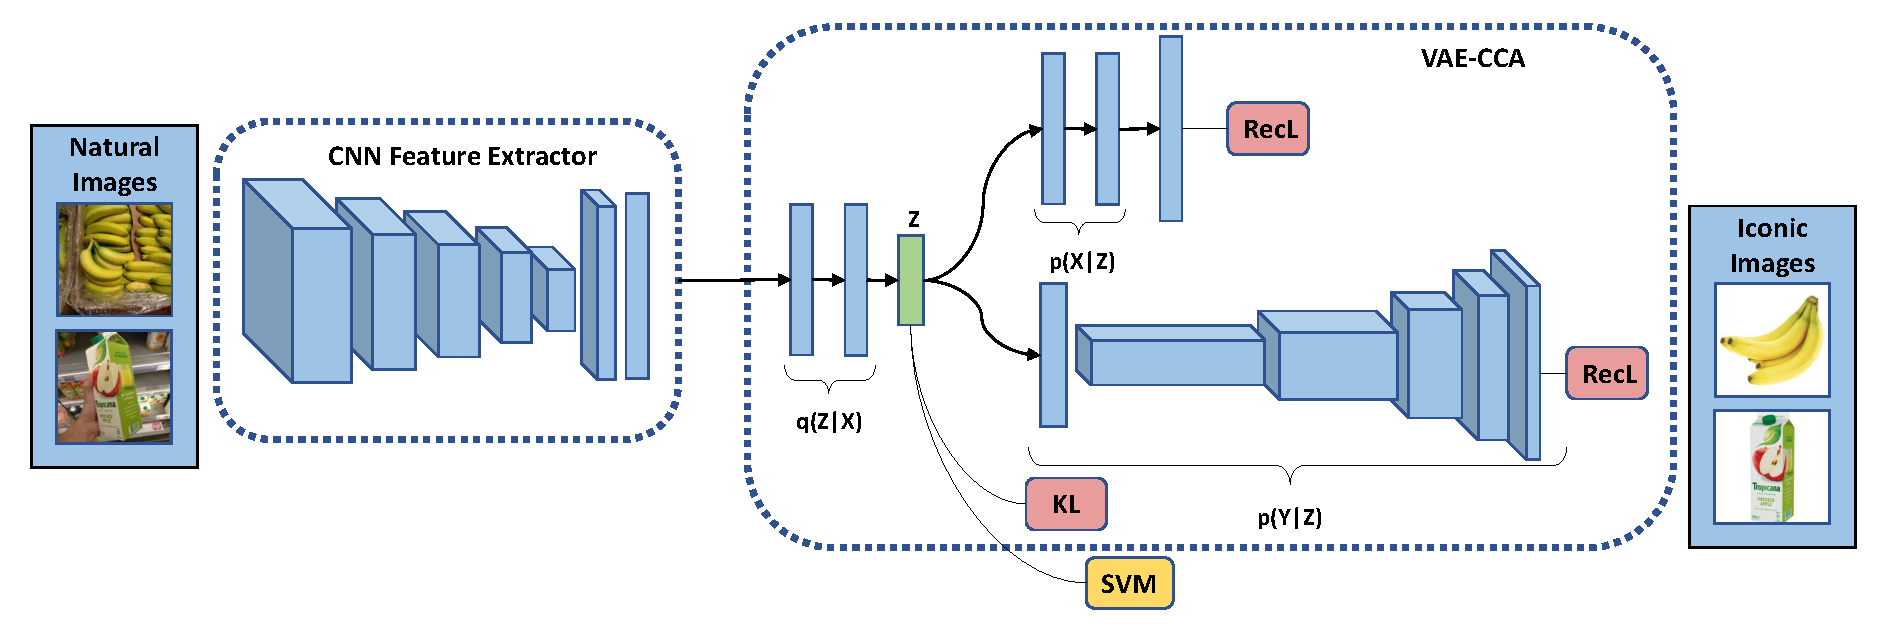
\includegraphics[width=\textwidth]{PaperA/figures/vae-cca.pdf}
		%\vspace{-7mm}
		\caption{}
		\label{subfig:vae-cca}
	\end{subfigure}
    %\subfigure[CNN]{\label{subfig:cnn}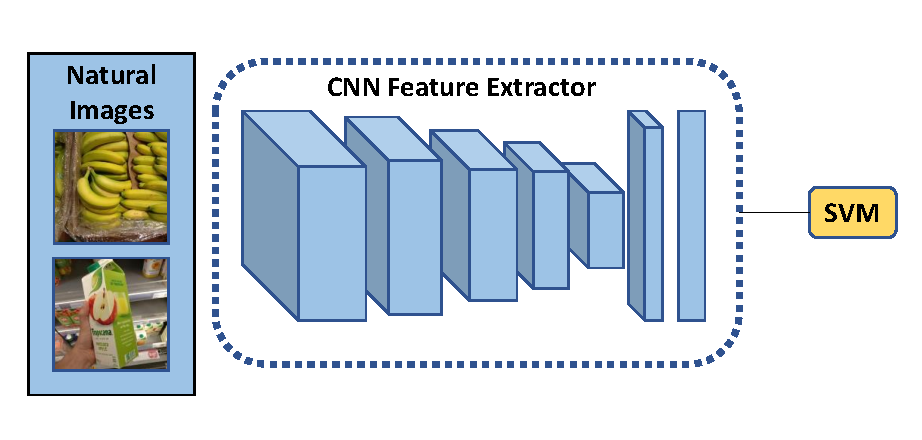
\includegraphics[width=0.35\textwidth]{PaperA/figures/cnn.pdf}} 
    %\subfigure[VAE]{\label{subfig:cnn+vae}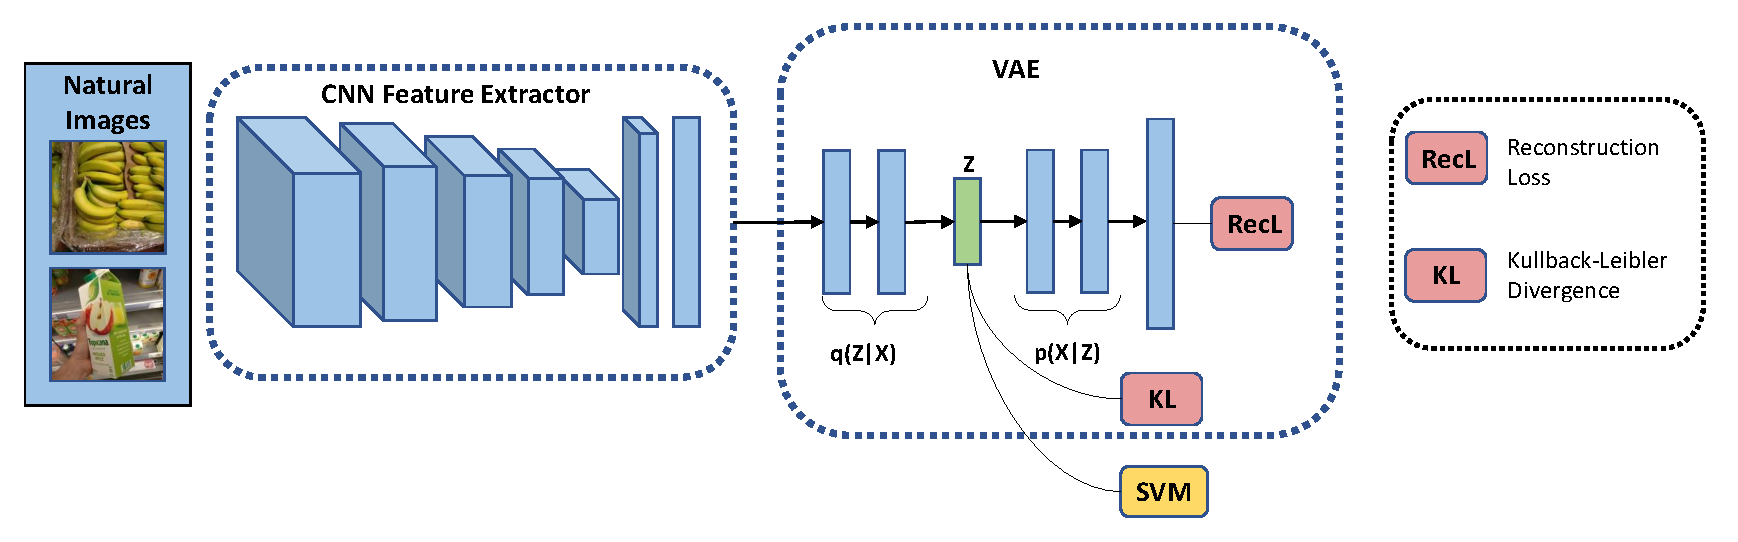
\includegraphics[width=0.6\textwidth]{PaperA/figures/cnn+vae.pdf}}
    %\subfigure[VAE-CCA]{\label{subfig:vae-cca}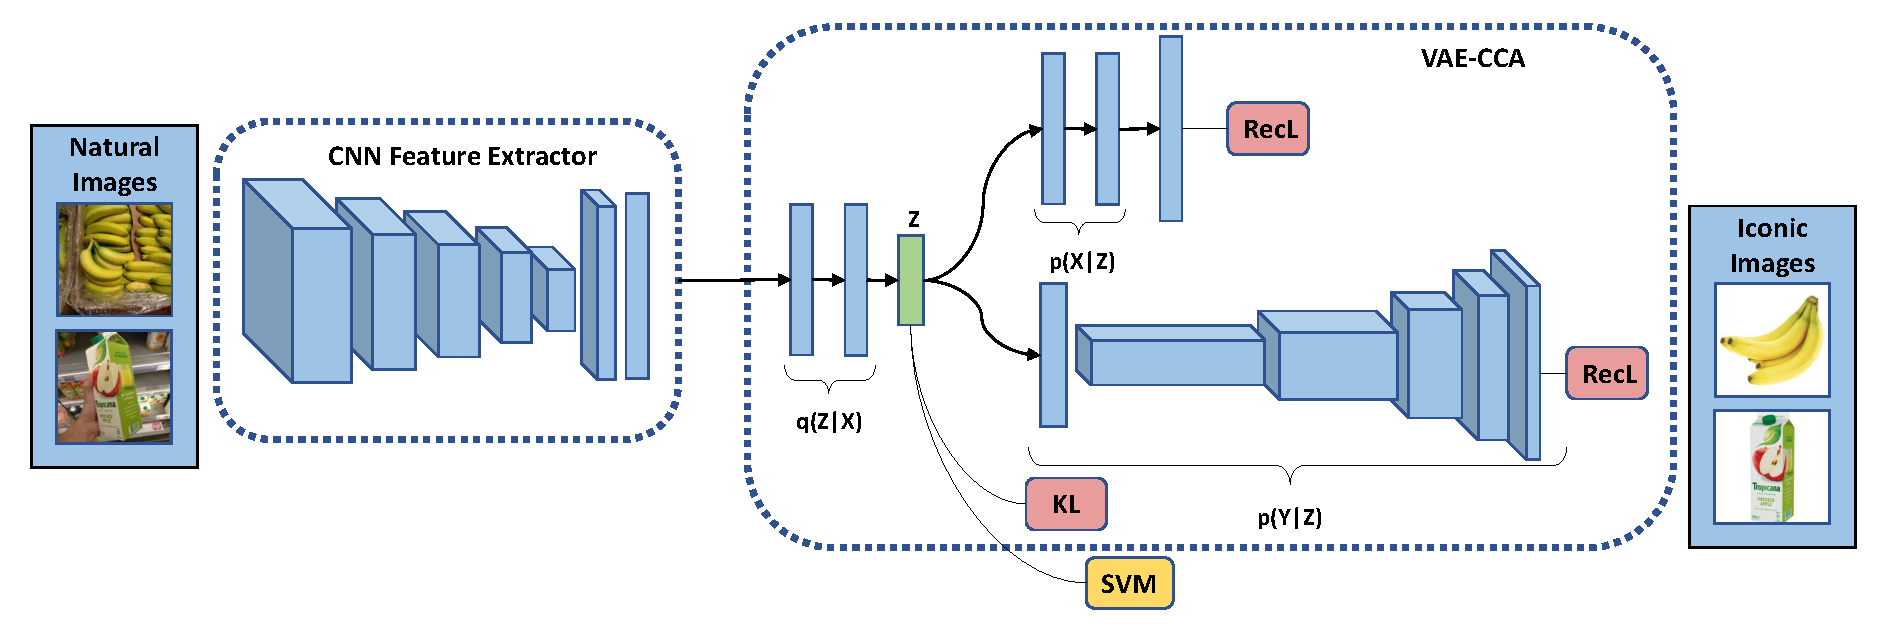
\includegraphics[width=0.7\textwidth]{PaperA/figures/vae-cca.pdf}}
    \caption{The architectures for the classification methods described in Section \ref{paperA:sec:classification-methods}. In this paper, we use either a pretrained AlexNet, VGG16 or DenseNet-169 as the CNN feature extractor, but it may be replaced with any CNN architecture. Note that the pretrained CNN can be fine-tuned. The encoder and decoder of the VAE in \ref{subfig:cnn+vae} consist of two fully-connected layers. VAE-CCA in \ref{subfig:vae-cca} uses the DCGAN architecture as an iconic image decoder and the same encoder and feature vector decoder as the VAE.   }
    \label{fig:classification-methods}
\end{figure}

%\end{comment}